% Options for packages loaded elsewhere
\PassOptionsToPackage{unicode}{hyperref}
\PassOptionsToPackage{hyphens}{url}
\PassOptionsToPackage{dvipsnames,svgnames,x11names}{xcolor}
%
\documentclass[
  11pt,
  a4paper,
]{article}

\usepackage{amsmath,amssymb}
\usepackage{setspace}
\usepackage{iftex}
\ifPDFTeX
  \usepackage[T1]{fontenc}
  \usepackage[utf8]{inputenc}
  \usepackage{textcomp} % provide euro and other symbols
\else % if luatex or xetex
  \usepackage{unicode-math}
  \defaultfontfeatures{Scale=MatchLowercase}
  \defaultfontfeatures[\rmfamily]{Ligatures=TeX,Scale=1}
\fi
\usepackage{lmodern}
\ifPDFTeX\else  
    % xetex/luatex font selection
    \setmainfont[]{Latin Modern Roman}
    \setsansfont[]{Latin Modern Roman}
\fi
% Use upquote if available, for straight quotes in verbatim environments
\IfFileExists{upquote.sty}{\usepackage{upquote}}{}
\IfFileExists{microtype.sty}{% use microtype if available
  \usepackage[]{microtype}
  \UseMicrotypeSet[protrusion]{basicmath} % disable protrusion for tt fonts
}{}
\usepackage{xcolor}
\usepackage[top=2.5cm,bottom=2.5cm,left=2.5cm,right=2.5cm]{geometry}
\setlength{\emergencystretch}{3em} % prevent overfull lines
\setcounter{secnumdepth}{5}
% Make \paragraph and \subparagraph free-standing
\makeatletter
\ifx\paragraph\undefined\else
  \let\oldparagraph\paragraph
  \renewcommand{\paragraph}{
    \@ifstar
      \xxxParagraphStar
      \xxxParagraphNoStar
  }
  \newcommand{\xxxParagraphStar}[1]{\oldparagraph*{#1}\mbox{}}
  \newcommand{\xxxParagraphNoStar}[1]{\oldparagraph{#1}\mbox{}}
\fi
\ifx\subparagraph\undefined\else
  \let\oldsubparagraph\subparagraph
  \renewcommand{\subparagraph}{
    \@ifstar
      \xxxSubParagraphStar
      \xxxSubParagraphNoStar
  }
  \newcommand{\xxxSubParagraphStar}[1]{\oldsubparagraph*{#1}\mbox{}}
  \newcommand{\xxxSubParagraphNoStar}[1]{\oldsubparagraph{#1}\mbox{}}
\fi
\makeatother


\providecommand{\tightlist}{%
  \setlength{\itemsep}{0pt}\setlength{\parskip}{0pt}}\usepackage{longtable,booktabs,array}
\usepackage{calc} % for calculating minipage widths
% Correct order of tables after \paragraph or \subparagraph
\usepackage{etoolbox}
\makeatletter
\patchcmd\longtable{\par}{\if@noskipsec\mbox{}\fi\par}{}{}
\makeatother
% Allow footnotes in longtable head/foot
\IfFileExists{footnotehyper.sty}{\usepackage{footnotehyper}}{\usepackage{footnote}}
\makesavenoteenv{longtable}
\usepackage{graphicx}
\makeatletter
\def\maxwidth{\ifdim\Gin@nat@width>\linewidth\linewidth\else\Gin@nat@width\fi}
\def\maxheight{\ifdim\Gin@nat@height>\textheight\textheight\else\Gin@nat@height\fi}
\makeatother
% Scale images if necessary, so that they will not overflow the page
% margins by default, and it is still possible to overwrite the defaults
% using explicit options in \includegraphics[width, height, ...]{}
\setkeys{Gin}{width=\maxwidth,height=\maxheight,keepaspectratio}
% Set default figure placement to htbp
\makeatletter
\def\fps@figure{htbp}
\makeatother
% definitions for citeproc citations
\NewDocumentCommand\citeproctext{}{}
\NewDocumentCommand\citeproc{mm}{%
  \begingroup\def\citeproctext{#2}\cite{#1}\endgroup}
\makeatletter
 % allow citations to break across lines
 \let\@cite@ofmt\@firstofone
 % avoid brackets around text for \cite:
 \def\@biblabel#1{}
 \def\@cite#1#2{{#1\if@tempswa , #2\fi}}
\makeatother
\newlength{\cslhangindent}
\setlength{\cslhangindent}{1.5em}
\newlength{\csllabelwidth}
\setlength{\csllabelwidth}{3em}
\newenvironment{CSLReferences}[2] % #1 hanging-indent, #2 entry-spacing
 {\begin{list}{}{%
  \setlength{\itemindent}{0pt}
  \setlength{\leftmargin}{0pt}
  \setlength{\parsep}{0pt}
  % turn on hanging indent if param 1 is 1
  \ifodd #1
   \setlength{\leftmargin}{\cslhangindent}
   \setlength{\itemindent}{-1\cslhangindent}
  \fi
  % set entry spacing
  \setlength{\itemsep}{#2\baselineskip}}}
 {\end{list}}
\usepackage{calc}
\newcommand{\CSLBlock}[1]{\hfill\break\parbox[t]{\linewidth}{\strut\ignorespaces#1\strut}}
\newcommand{\CSLLeftMargin}[1]{\parbox[t]{\csllabelwidth}{\strut#1\strut}}
\newcommand{\CSLRightInline}[1]{\parbox[t]{\linewidth - \csllabelwidth}{\strut#1\strut}}
\newcommand{\CSLIndent}[1]{\hspace{\cslhangindent}#1}

\usepackage{booktabs}
\usepackage{longtable}
\usepackage{array}
\usepackage{multirow}
\usepackage{wrapfig}
\usepackage{float}
\usepackage{colortbl}
\usepackage{pdflscape}
\usepackage{tabu}
\usepackage{threeparttable}
\usepackage{threeparttablex}
\usepackage[normalem]{ulem}
\usepackage{makecell}
\usepackage{xcolor}
\usepackage{fancyhdr}
\usepackage{amsmath}
\usepackage{multirow}
\usepackage{booktabs}
\usepackage{pifont}
\makeatletter
\@ifpackageloaded{caption}{}{\usepackage{caption}}
\AtBeginDocument{%
\ifdefined\contentsname
  \renewcommand*\contentsname{Table of contents}
\else
  \newcommand\contentsname{Table of contents}
\fi
\ifdefined\listfigurename
  \renewcommand*\listfigurename{List of Figures}
\else
  \newcommand\listfigurename{List of Figures}
\fi
\ifdefined\listtablename
  \renewcommand*\listtablename{List of Tables}
\else
  \newcommand\listtablename{List of Tables}
\fi
\ifdefined\figurename
  \renewcommand*\figurename{Figure}
\else
  \newcommand\figurename{Figure}
\fi
\ifdefined\tablename
  \renewcommand*\tablename{Table}
\else
  \newcommand\tablename{Table}
\fi
}
\@ifpackageloaded{float}{}{\usepackage{float}}
\floatstyle{ruled}
\@ifundefined{c@chapter}{\newfloat{codelisting}{h}{lop}}{\newfloat{codelisting}{h}{lop}[chapter]}
\floatname{codelisting}{Listing}
\newcommand*\listoflistings{\listof{codelisting}{List of Listings}}
\makeatother
\makeatletter
\makeatother
\makeatletter
\@ifpackageloaded{caption}{}{\usepackage{caption}}
\@ifpackageloaded{subcaption}{}{\usepackage{subcaption}}
\makeatother

\ifLuaTeX
  \usepackage{selnolig}  % disable illegal ligatures
\fi
\usepackage{bookmark}

\IfFileExists{xurl.sty}{\usepackage{xurl}}{} % add URL line breaks if available
\urlstyle{same} % disable monospaced font for URLs
\hypersetup{
  pdftitle={Estimation of Effects of Endogenous Time-Varying Covariates: A Comparison Of Multilevel Linear Modeling and Generalized Estimating Equations},
  pdfauthor={Ward B. Eiling (9294163)},
  colorlinks=true,
  linkcolor={blue},
  filecolor={Maroon},
  citecolor={Blue},
  urlcolor={Blue},
  pdfcreator={LaTeX via pandoc}}


\title{Estimation of Effects of Endogenous Time-Varying Covariates: A
Comparison Of Multilevel Linear Modeling and Generalized Estimating
Equations}
\usepackage{etoolbox}
\makeatletter
\providecommand{\subtitle}[1]{% add subtitle to \maketitle
  \apptocmd{\@title}{\par {\large #1 \par}}{}{}
}
\makeatother
\subtitle{Research Report}
\author{Ward B. Eiling (9294163)}
\date{December 16, 2024}

\begin{document}
\cleardoublepage
\thispagestyle{empty}
{\centering
\hbox{}\vskip 0cm plus 1fill
% \vspace{25ex}
{\Large\bfseries Estimation of Effects of Endogenous Time-Varying
Covariates: A Comparison Of Multilevel Linear Modeling and Generalized
Estimating Equations \par}
\vspace{3ex}
{\large Research Report \par}
\vspace{9ex}
{\large\bfseries Ward B. Eiling (9294163) \par}
\vspace{3ex}
% {\Large ORCID: 0009-0007-8114-9497 \par}
% \vspace{3ex}
{\large Supervisors: Ellen Hamaker and Jeroen Mulder \par}
% \vskip 0cm plus 2fill
\vspace{9ex}
{\normalsize \textit{Master's degree in Methodology and Statistics for the Behavioural, \\ Biomedical and Social Sciences} \par}
\vspace{3ex}
{\normalsize \textit{Utrecht University} \par}
\vspace{9ex}
{\normalsize December 16, 2024 \par}
\vspace{3ex}
{\normalsize Word count: 2500/2500 \par}
\vspace{9ex}
{\normalsize FETC-approved: 24-2003 \par}
\vspace{9ex}
{\normalsize \textit{Candidate journal: Psychological Methods} \par}
\hbox{}\vskip 0cm plus 1fill
% \vspace{12ex}
% %
% %
% {\large Utrecht University \par}
% %
% %
% {\large Methodology and Statistics \par}
% \vspace{3ex}
% %
% {\large  \par}
% %
% \vspace{12ex}
% {\small Submitted in total fulfilment of the requirements
% of the degree of Doctor of Philosophy \par}
}


\setstretch{2}
\newpage

\section{Introduction}\label{introduction}

Across a wide range of disciplines, researchers analyze clustered
longitudinal, observational data to investigate prospective causal
relationships between variables. When analyzing such data, psychological
researchers most commonly use the multilevel linear model\footnote{The
  MLM is known by various names, including: linear mixed model,
  hierarchical linear model, random-effect model and mixed-effects
  model.} (MLM, \citeproc{ref-bauer2011}{Bauer \& Sterba, 2011}),
which---in the context of longitudinal data analysis---partitions
observed variance into stable between-person differences and
within-person fluctuations (\citeproc{ref-hamaker2020}{Hamaker \&
Muthén, 2020}). In the application of the MLM, time invariant and
time-varying covariates, the latter measured repeatedly over time, are
often available. The inclusion of covariates is a common strategy to
improve parameter precision and address bias introduced by
(time-varying) confounders (\citeproc{ref-daniel2013}{Daniel et al.,
2013}; \citeproc{ref-Wodtke2020}{Wodtke, 2020}). Nevertheless, it is
well-known that this approach is not universally beneficial, as
conditioning on variables like colliders within the causal pathway can
distort treatment effect estimates (\citeproc{ref-elwert2014}{Elwert \&
Winship, 2014}).

Dating back to the work of Pepe and Anderson (1994), it has been
well-established that including endogenous time-varying
covariates---those directly or indirectly influenced by prior
exposure/treatment or outcome---in longitudinal studies without
treatment can result in biased estimates of treatment effects. Despite
its significance, this issue has received little attention in
psychological research. Building on this foundation, a recent paper by
Qian et al.~(2020) examined the suitability of MLM for estimating the
causal effect of a time-varying exposure or treatment. Specifically,
they focused on settings where the exposure is randomly assigned at each
occasion within individuals. Such randomized exposures may include, for
example, prompts delivered through push notifications to remind
participants of cognitive or mindfulness-based strategies
(\citeproc{ref-nahum-shani2021}{Nahum-Shani et al., 2021};
\citeproc{ref-walton2018}{Walton et al., 2018}). While random assignment
with a constant probability might seem sufficient to identify (the
presence and absence of) causal effects, Qian et al.
(\citeproc{ref-qian2020}{2020}) showed that model fitting issues and
parameter bias can arise when a \emph{time-varying endogenous covariate}
is present.

However, due to a divide between the disciplines that employ the MLM,
such critiques appear to have largely failed to reach the applied
researcher in psychology. One specific reason might be that the
technical jargon in other disciplines makes it difficult for researchers
to recognize when and how these issues emerge. Therefore, this report
aims to understand why Qian et al. (\citeproc{ref-qian2020}{2020}) found
biased estimates of the treatment effect for some generative models
containing endogenous covariates and not for others; and to explain this
issue to an audience of psychologists. To achieve this aim, the study
will first use graphical diagrams to evaluate relevant criteria,
ensuring accessibility and rigor through a reliance on graphical rules
rather than algebra. Next, data simulations, based on the original
scenarios of Qian et al. (\citeproc{ref-qian2020}{2020}) as well as
additional scenarios, will be conducted to pinpoint the issue and to
assess whether these criteria effectively identify bias. Accordingly,
the following research question will be addressed: \emph{When does the
inclusion of endogenous variables in multilevel linear models result in
biased estimates of the treatment effect?}

\section{Methods}\label{methods}

To obtain a better understanding of the issue exposed by Qian et al.
(\citeproc{ref-qian2020}{2020}), two methods were employed. First,
graphical methods were used provide insight into the presence and extent
of bias with potential violation of criteria: (a) path diagrams were
used to evaluate the conditional independence assumption
(\citeproc{ref-qian2020}{Qian et al., 2020}) and (b) directed acyclic
graphs (DAGs) were used to evaluate the backdoor criterion
(\citeproc{ref-pearl1988}{Pearl, 1988}, \citeproc{ref-pearl2009}{2009}).
Second, a simulation study was performed to reproduce the results for
the generative models (GMs) from Qian et al.
(\citeproc{ref-qian2020}{2020}) and to further isolate the issue using
additional GMs. In this simulation, bias in the treatment effect was
quantified using analytical multilevel models identical to the
generative models.

\subsection{Data Generation}\label{data-generation}

We consider 2 generative models (GMs) from Qian et al.
(\citeproc{ref-qian2020}{2020}), one (GM A) being a special case of the
general model (GM G) where bias was detected. To further isolate the
source of bias, we introduce two additional special cases, labeled GM B
and C. Table~\ref{tbl-gm-differences} summarizes the differences between
the generative models. Compared to the general model G, GM A is not
directly determined by the random intercept \(b_{i0}\); GM B is does not
have a random slope \(b_{i2}\) for treatment; and GM C does not have a
fixed interaction effect \(\beta_1\) between covariate and treatment.

\begin{longtable}[]{@{}
  >{\raggedright\arraybackslash}p{(\columnwidth - 8\tabcolsep) * \real{0.2000}}
  >{\raggedright\arraybackslash}p{(\columnwidth - 8\tabcolsep) * \real{0.2000}}
  >{\raggedright\arraybackslash}p{(\columnwidth - 8\tabcolsep) * \real{0.2000}}
  >{\raggedright\arraybackslash}p{(\columnwidth - 8\tabcolsep) * \real{0.2000}}
  >{\raggedright\arraybackslash}p{(\columnwidth - 8\tabcolsep) * \real{0.2000}}@{}}
\caption{Generative Models: Summary of
Differences}\label{tbl-gm-differences}\tabularnewline
\toprule\noalign{}
\begin{minipage}[b]{\linewidth}\raggedright
Generative Model
\end{minipage} & \begin{minipage}[b]{\linewidth}\raggedright
Name in Qian et al. (\citeproc{ref-qian2020}{2020})
\end{minipage} & \begin{minipage}[b]{\linewidth}\raggedright
dependency \(b_{i0}\) and \(X_{it}\)
\end{minipage} & \begin{minipage}[b]{\linewidth}\raggedright
random slope treatment \(b_{i2}\)
\end{minipage} & \begin{minipage}[b]{\linewidth}\raggedright
interaction \(\beta_1\)
\end{minipage} \\
\midrule\noalign{}
\endfirsthead
\toprule\noalign{}
\begin{minipage}[b]{\linewidth}\raggedright
Generative Model
\end{minipage} & \begin{minipage}[b]{\linewidth}\raggedright
Name in Qian et al. (\citeproc{ref-qian2020}{2020})
\end{minipage} & \begin{minipage}[b]{\linewidth}\raggedright
dependency \(b_{i0}\) and \(X_{it}\)
\end{minipage} & \begin{minipage}[b]{\linewidth}\raggedright
random slope treatment \(b_{i2}\)
\end{minipage} & \begin{minipage}[b]{\linewidth}\raggedright
interaction \(\beta_1\)
\end{minipage} \\
\midrule\noalign{}
\endhead
\bottomrule\noalign{}
\endlastfoot
G(eneral) & 3 & \(\checkmark\) & \(\checkmark\) & \(\checkmark\) \\
A & 1 & \(\times\) & \(\checkmark\) & \(\checkmark\) \\
B & NA & \(\checkmark\) & \(\times\) & \(\checkmark\) \\
C & NA & \(\checkmark\) & \(\checkmark\) & \(\times\) \\
\end{longtable}

The details of the generative models are described below. We follow the
symbol notation of Qian et al. (\citeproc{ref-qian2020}{2020}) to allow
for direct comparison, but rewrite the equations into within- and
between-person models (see \citeproc{ref-raudenbush2002}{Raudenbush \&
Bryk, 2002}; \citeproc{ref-Schoot2017}{Schoot, 2017}).

\subsubsection{Generative Model G}\label{generative-model-g}

Following the original notation of Qian et al.
(\citeproc{ref-qian2020}{2020}), the outcome of GM G was generated
according to the following model:

\[
Y_{it+1} = \alpha_0 + \alpha_1 X_{it} + b_{i0} + A_{it} (\beta_0 + \beta_1 X_{it} + b_{i2}) + \epsilon_{it+1}
\]

where \(Y_{it+1}\) is the outcome at time \(t+1\), \(X_{it}\) is the
covariate at time \(t\), \(A_{it}\) is the treatment at time \(t\),
\(b_{i0}\) is the random intercept, \(b_{i2}\) is the random slope for
the treatment, and \(\epsilon_{it+1}\) is the error term. We may rewrite
this model into the repeated-observations or within-person model in the
following steps:

\[ 
\begin{aligned} Y_{it+1} &= \alpha_0 + \alpha_1 X_{it} + b_{i0} + A_{it} (\beta_0 + \beta_1 X_{it} + b_{i2}) + \epsilon_{it+1} \\ &= \alpha_0 + \alpha_1 X_{it} + b_{i0} + \beta_0 A_{it} +  \beta_1 A_{it} X_{it} + A_{it} b_{i2} + \epsilon_{it+1} \\ &= \alpha_0 + b_{i0} + \alpha_1 X_{it} + \beta_0 A_{it} + A_{it} b_{i2} + \beta_1 A_{it} X_{it} + \epsilon_{it+1} \\ &= (\alpha_0 + b_{i0}) + \alpha_1 X_{it} + (\beta_0 + b_{i2}) A_{it} + \beta_1 A_{it} X_{it} + \epsilon_{it+1} \\ &= \pi_{0i} + \pi_{1i} X_{it} + \pi_{2i} A_{it} + \pi_{3i} A_{it} X_{it} + \epsilon_{it+1}. \end{aligned}
\]

with the person-level or between-person model (level 2):

\[
\begin{aligned}
\pi_{0i} &= \alpha_0 + b_{i0}, & \text{where} \quad b_{i0} &\sim \mathcal{N}(0, \sigma_{b0}^2), \\
\pi_{1i} &= \alpha_1, \\
\pi_{2i} &= \beta_0 + b_{i2}, & \text{where} \quad b_{i2} &\sim \mathcal{N}(0, \sigma_{b2}^2), \\
\pi_{3i} &= \beta_1.
\end{aligned}
\]

We model fixed effects \(\alpha_0\), \(\alpha_1\), \(\beta_0\), and
\(\beta_1\) as constants across individuals, while random effects
\(b_{i0}\) and \(b_{i2}\) capture individual-specific deviations.
Specifically, \(b_{i0}\) represents deviations from the population
intercept \(\alpha_0\), and \(b_{i2}\) represents deviations from the
population slope \(\beta_0\). A higher \(b_{i0}\) indicates a higher
initial outcome, while a higher \(b_{i2}\) indicates a stronger
treatment effect. Following Qian et al. (\citeproc{ref-qian2020}{2020}),
the random effects \(b_{i0}\) and \(b_{i2}\) are modeled independent of
each other.

The covariate is generated as:

\[
X_{it} = 
\begin{cases} 
b_{i0} + \epsilon_{X_{it}}, & \text{if } t = 1, \\
b_{i0} + Y_{it} + \epsilon_{X_{it}}, & \text{if } t \geq 2,
\end{cases}
\quad \text{where} \quad \epsilon_{X_{it}} \sim \mathcal{N}(0, 1)
\]

The randomization probability of treatment
\(p_t = P(A_{it} = 1 \mid H_{it})\) is constant at \(1/2\). Thus,
\(A_{it} \sim \text{Bernoulli}(0.5)\) for \(i = 1, \ldots, N\) and
\(t = 1, \ldots, T\). In other words, for every given person \(i\) and
every timepoint \(t\), the probability that treatment is assigned is
equivalent to a fair coinflip. The exogenous noise is
\(\epsilon_{it+1} \sim \mathcal{N}(0, \sigma_\epsilon^2)\).

Figure~\ref{fig-GMG_path} shows the path diagram for the first couple
observations of GM G.

\subsubsection{Generative Model A}\label{generative-model-a}

GM A is a special case of GM G, where the effect of the random intercept
\(b_{i0}\) on the covariate \(X_{it}\) is set to zero. This results in a
model where the covariate \(X_{it}\) is not directly determined by the
random intercept \(b_{i0}\) (see Figure~\ref{fig-GMA_path}). Instead,
the endogenous covariate \(X_{it}\) equals the previous outcome
\(Y_{it}\) plus some random noise:

\[
X_{it} = 
\begin{cases} 
\epsilon_{X_{it}}, & \text{if } t = 1, \\
Y_{it} + \epsilon_{X_{it}}, & \text{if } t \geq 2,
\end{cases}
\quad \text{where} \quad \epsilon_{X_{it}} \sim \mathcal{N}(0, 1)
\]

\subsubsection{Generative Model B}\label{generative-model-b}

GM B is a special case of GM G, where the variance for the random slope
\(b_{i2}\) is set to zero: \(\sigma_{b2}^2\) = 0. Consequently, the
random slope \(b_{i2}\) for the treatment \(A_{it}\) is removed (see
Figure~\ref{fig-GMB_path}). While the within-person model is the same as
GM G, there is a slight alteration in the between-person model:

\[ \pi_{2i} = \beta_0. \]

The single equation model then becomes:

\[
Y_{it+1} = (\alpha_0 + b_{i0}) + \alpha_1 X_{it} + \beta_0 A_{it} + \beta_1 A_{it} X_{it} + \epsilon_{it+1}
\]

\subsubsection{Generative Model C}\label{generative-model-c}

GM C is a special case of GM G, where the fixed interaction parameter
\(\beta_1 = 0\), which implies the removal of the interaction term
\(\beta_1 A_{it} X_{it}\) (see Figure~\ref{fig-GMC_path}). This, in
turn, removed \(\pi_{3i}\), thereby creating a discrepancy in
within-person model of GM C and GM G:

\[Y_{it+1} = \pi_{0i} + \pi_{1i} X_{it} + \pi_{2i} A_{it} + \epsilon_{it+1}.\]

Nevertheless, the between-person model of \(\pi_{0i}\), \(\pi_{1i}\) and
\(\pi_{2i}\) remains the same as GM G. The single equation model then
becomes:

\[
Y_{it+1} = \alpha_0 + \alpha_1 X_{it} + b_{i0} + A_{it} (\beta_0 + b_{i2}) + \epsilon_{it+1}.
\]

\subsubsection{Parameter Values}\label{parameter-values}

The following parameter values were adapted from Qian et al.
(\citeproc{ref-qian2020}{2020}):

\[
\alpha_0 = -2, \quad \alpha_1 = -0.3, \quad \beta_0 = 1, \quad \beta_1 = 0.3,
\]

\[
\sigma_{b0}^2 = 4, \quad \sigma_{b2}^2 = 1, \quad \sigma_\epsilon^2 = 1.
\]

\subsection{Data Analysis}\label{data-analysis}

In the simulation study, we evaluated the performance of the models
across a total of 24 different settings, each replicated 1,000 times, by
systematically varying the following factors:

\begin{itemize}
\item
  \textbf{Generative Models (GM):} G, A, B, C
\item
  \textbf{Number of timepoints (T):} 10, 30
\item
  \textbf{Sample size (N):} 30, 100, 200
\end{itemize}

All data generation and estimation was performed in \texttt{R}, version
4.4.2 (\citeproc{ref-rcoreteam2024}{Team, 2024}). After the generation
of data generation for any given setting, analytical multilevel linear
models were fit that are equivalent to each of the respective
data-generating models. To fit the standard MLM, the \texttt{lmer}
function from the R-package \texttt{lme4}
(\citeproc{ref-bates2015}{Bates et al., 2015}) was employed with
restricted maximum likelihood estimation.

\section{Results}\label{results}

\subsection{Conditional Independence and Path
Diagrams}\label{conditional-independence-and-path-diagrams}

The first criterion to evaluate the presence of bias in the treatment
effect estimates is the \emph{conditional independence assumption}.
According to Qian et al. (\citeproc{ref-qian2020}{2020}), this
assumption should identify whether estimators of the treatment effect
are consistent and unbiased under randomized treatment assignment. The
conditional independence assumption states that the covariate at time
\(t\) (\(X_{it}\)) should be independent of the individual's random
effects (\(b_{i0}\) and \(b_{i1}\)) once we account for their history of
covariates (\(H_{it-1}\)), previous treatments (\(A_{it-1}\)), and prior
outcomes (\(Y_{it}\)). This is implied from the following notation:

\[ 
X_{it} \perp (b_{i0}, b_{i1}) \mid H_{it-1}, A_{it-1}, Y_{it}.
\]

where \(b_{i0}\) and \(b_{i1}\) represent the random intercept and
random slope(s), respectively, and \(H_{it-1}\) comprises all
observations of that covariate before timepoint \(t\). This assumption
allows for \(X_{it}\) to be influenced by earlier variables (e.g.,
outcomes or treatments) but not directly by unobserved individual
characteristics (i.e., random effects). If the included endogenous
covariates are only affected by prior outcomes and treatments, the
assumption is automatically satisfied. However, as Qian et al.
(\citeproc{ref-qian2020}{2020}) highlights, ensuring this assumption
holds requires careful consideration of theory and domain knowledge.

To clarify the application of the conditional independence assumption,
we pair the equations of the generative models (GMs) with path diagrams
(\citeproc{ref-duncan1966}{Duncan, 1966};
\citeproc{ref-wright1934a}{Wright, 1934}) illustrating the first three
timepoints (\(t\)) for each model (see Figure~\ref{fig-Pathdiagrams}).

\begin{figure}[H]

\caption{\label{fig-Pathdiagrams}Path Diagrams for Generative Models G,
A, B and C (t = 1, 2, 3)}

\begin{minipage}{0.50\linewidth}

\subcaption{\label{fig-GMG_path}GM G}

\centering{

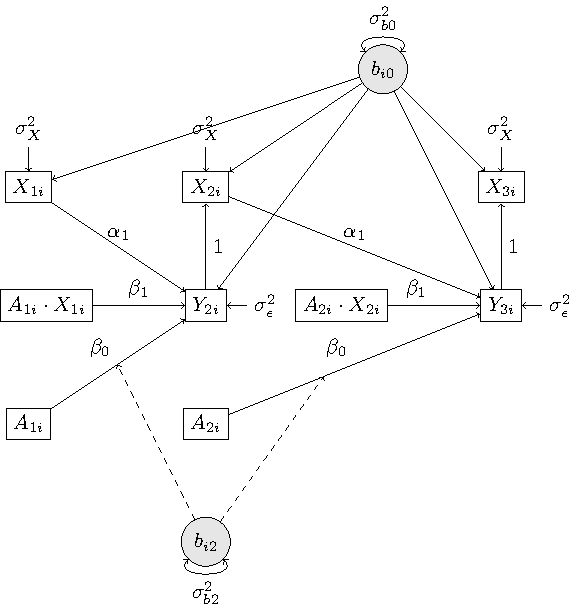
\includegraphics[width=1\textwidth,height=\textheight]{research-report_files/figure-pdf/fig-GMG_path-1.pdf}

}

\end{minipage}%
%
\begin{minipage}{0.50\linewidth}

\subcaption{\label{fig-GMA_path}GM A}

\centering{

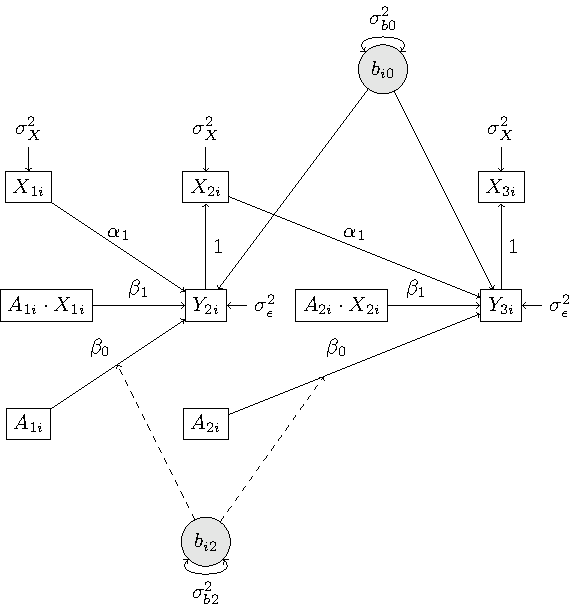
\includegraphics[width=1\textwidth,height=\textheight]{research-report_files/figure-pdf/fig-GMA_path-1.pdf}

}

\end{minipage}%
\newline
\begin{minipage}{0.50\linewidth}

\subcaption{\label{fig-GMB_path}GM B}

\centering{

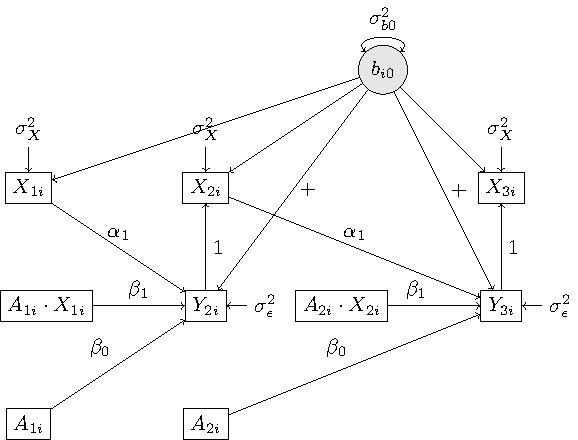
\includegraphics[width=1\textwidth,height=\textheight]{research-report_files/figure-pdf/fig-GMB_path-1.pdf}

}

\end{minipage}%
%
\begin{minipage}{0.50\linewidth}

\subcaption{\label{fig-GMC_path}GM C}

\centering{

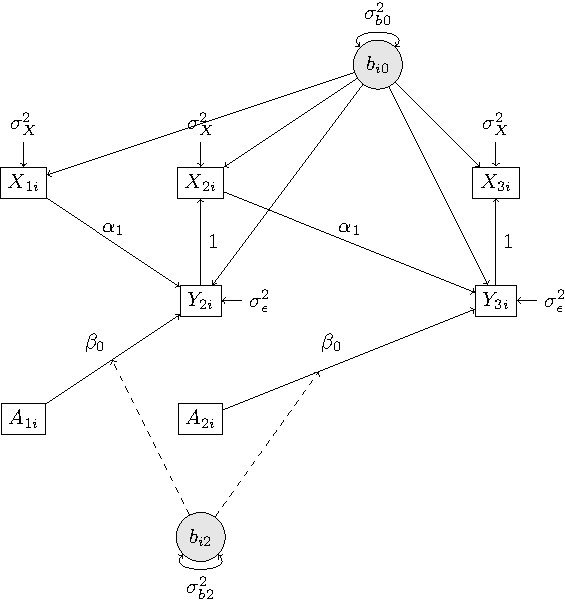
\includegraphics[width=1\textwidth,height=\textheight]{research-report_files/figure-pdf/fig-GMC_path-1.pdf}

}

\end{minipage}%

\end{figure}%

\emph{Note.} Random effects are represented by grey circles, observed
variables by squares and relationships across variables by arrows, where
dashed lines are reserved for random slopes.

\vspace{2em}

Let's begin with the general model, GM G (Figure~\ref{fig-GMG_path}),
which Qian et al. (\citeproc{ref-qian2020}{2020}) identified as prone to
bias. In GM G, the covariate \(X_{it}\) is directly influenced by
unobserved individual factors (represented by the random effects,
\(b_{i0}\)). Consequently, conditioning on prior variables, such as the
outcome at the previous timepoint \(Y_{it}\), does not fully block or
eliminate the influence of these unobserved factors. As a result,
\(X_{it}\) remains dependent on the random effects, violating the
assumption that \(X_{it}\) should be independent of these unobserved
factors once we account for prior variables. This violation of the
conditional independence assumption explains the biased estimates of the
treatment effect observed in GM G, as identified by Qian et al.
(\citeproc{ref-qian2020}{2020}).

In contrast, GM A, a special case of GM G where no bias was found by
Qian et al. (\citeproc{ref-qian2020}{2020}), removes the direct link
between \(X_{it}\) and the random effects \(b_{i0}\). In this case,
\(X_{it}\) is simply the previous outcome \(Y_{it}\) plus some random
noise. While there remains an indirect connection between \(X_{it}\) and
\(b_{i0}\) through \(Y_{it}\), conditioning on \(Y_{it}\) effectively
``breaks the link'' between \(X_{it}\) and the random effects,
satisfying the conditional independence assumption. This explains the
unbiased treatment effect estimates found by Qian et al.
(\citeproc{ref-qian2020}{2020}).

For the additional special cases, GM B and GM C, the direct link between
the random effects and \(X_{it}\) remains, as in GM G. As a result,
these models also violate the conditional independence assumption,
leading to biased estimates of the treatment effect.

In summary, GM G, B, and C violate the conditional independence
assumption, which suggests that we would expect biased treatment effect
estimates for these models. In contrast, GM A satisfies the assumption,
supporting unbiased estimates of the treatment effect.

\subsection{Backdoor Criterion and
DAGs}\label{backdoor-criterion-and-dags}

The second criterion for evaluating the presence of bias in treatment
effect estimates is the \emph{backdoor criterion}
(\citeproc{ref-pearl1988}{Pearl, 1988}, \citeproc{ref-pearl2009}{2009}).
This criterion provides a partial solution to the classical problem in
causal inference: \emph{causal effects} cannot be directly observed and
must instead be inferred from observed associations, which often
represent a mixture of causal effects and various undesirable
non-causal, or \emph{spurious}, components
(\citeproc{ref-Holland1986}{Holland, 1986}). When it is possible, under
ideal conditions (e.g., no measurement error, infinite sample size), to
isolate the causal effect from a combination of causal and spurious
components, the causal effect is said to be identified. According to the
backdoor criterion (\citeproc{ref-pearl1988}{Pearl, 1988},
\citeproc{ref-pearl2009}{2009}), causal effects can be identified by
blocking non-causal paths through conditioning on appropriate variables
(e.g., controlling or matching). For instance, a causal effect of
exposure on outcome can be identified by including in the analysis
(i.e., controlling for) all relevant confounders---common causes that
would otherwise induce spurious relationships. However, if spurious
paths remain unblocked due to unmeasured variables or measurement error,
the treatment and outcome remain linked via backdoor paths, leading to
biased estimates of the treatment effect (\citeproc{ref-Kim2021a}{Kim \&
Steiner, 2021}).

To detect the presence of such backdoor paths, directed acyclic graphs
(DAGs) (\citeproc{ref-pearl1995}{Pearl, 1995},
\citeproc{ref-pearl2009}{2009}) are invaluable tools. DAGs generalize
conventional linear path diagrams (\citeproc{ref-duncan1966}{Duncan,
1966}; \citeproc{ref-wright1934a}{Wright, 1934}) and operate in a fully
nonparametric framework. Unlike traditional path diagrams, DAGs make no
assumptions about distributional properties (e.g., multivariate
normality) or functional forms (e.g., linearity). Instead, they encode
qualitative causal assumptions about the data-generating process in the
population. Arrows connecting nodes indicate direct causal effects,
which may vary in magnitude across individuals (effect heterogeneity) or
depend on the values of other variables (effect interaction or
modification) (\citeproc{ref-elwert2014}{Elwert \& Winship, 2014}).
Notably, random slopes from random-effects models and interaction
effects are not explicitly represented in DAGs, which precludes their
use for evaluating the conditional independence assumption.

Using the direct causal effects specified in each generative model (GM),
we can formulate DAGs for the first three observations, representing the
random disturbance \(b_{0i}\) as the node \(U\) (e.g.,
\citeproc{ref-Kim2021a}{Kim \& Steiner, 2021}, see
Figure~\ref{fig-DAGs}). These diagrams confirm that random slopes and
fixed interaction effects are absent. Indeed, this absence explains why
the DAGs for GMs G, B, and C are equivalent.

\begin{figure}[H]

\caption{\label{fig-DAGs}DAGs for Generative Models G, A, B and C (t =
1, 2, 3)}

\begin{minipage}{0.50\linewidth}

\subcaption{\label{fig-GMG_DAG}GM G, B, C}

\centering{

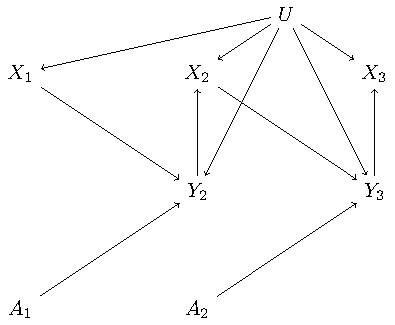
\includegraphics{research-report_files/figure-pdf/fig-GMG_DAG-1.pdf}

}

\end{minipage}%
%
\begin{minipage}{0.50\linewidth}

\subcaption{\label{fig-GMA_DAG}GM A}

\centering{

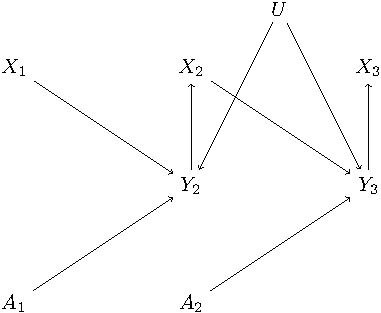
\includegraphics{research-report_files/figure-pdf/fig-GMA_DAG-1.pdf}

}

\end{minipage}%

\end{figure}%

\emph{Note.} The red arrows show the biased backdoor path(s) in the
treatment efffect (before controlling for \(X_{it}\)).

\vspace{2em}

We now apply the backdoor criterion to these DAGs to assess potential
bias in the treatment effect. For all GMs, there are no backdoor paths
in the treatment effect \(A_t \to Y_{t+1}\), as \(A_t\) lacks any parent
nodes. Consequently, covariate \(X_t\) need not be controlled to obtain
an unbiased total effect. Importantly, including \(X_{it}\) does not
introduce identification issues, as it is neither a mediator (i.e., on
the pathway from \(A_t\) to \(Y_{t+1}\)) nor a collider (i.e., a common
effect of \(A_t\) and \(Y_{t+1}\)). Therefore, according to the backdoor
criterion, controlling for \(X_{it}\) should not result in biased
estimates of the treatment effect in any of the generative models.

\subsection{Simulation Study}\label{simulation-study}

Table~\ref{tbl-simulation-results} and
Figure~\ref{fig-simulation-results} present the simulation results for
each of the generative models. The \(\beta_0\) bias in
Table~\ref{tbl-simulation-results} refers to
\(\bar{\hat{\beta}}_{0} - \beta_{0}\), representing the difference
between the mean of the estimated parameter values
\(\bar{\hat{\beta}}_{0}\) and the prespecified treatment effect
\(\beta_{0} = 1\). Thus, an absolute bias of 0.05 implies a \(5\%\)
relative bias.

\begin{table}

\caption{\label{tbl-simulation-results}Treatment effect bias for
Generative Models G, A, B and C over 1000 replications}

\centering{

\begin{tabu} to \linewidth {>{\raggedright\arraybackslash}p{5em}>{\raggedleft}X>{\raggedleft}X>{\raggedleft}X>{\raggedleft}X>{\raggedleft}X}
\toprule
\multicolumn{3}{c}{ } & \multicolumn{2}{c}{$\beta_0$} & \multicolumn{1}{c}{ } \\
\cmidrule(l{3pt}r{3pt}){4-5}
GM & T & N & Bias & SD & SR\\
\midrule
 &  & 30 & -0.052 & 0.245 & 0.999\\
\cmidrule{3-6}
 &  & 100 & -0.064 & 0.134 & 1.000\\
\cmidrule{3-6}
 & \multirow{-3}{*}{\raggedleft\arraybackslash 10} & 200 & -0.051 & 0.096 & 1.000\\
\cmidrule{2-6}
 &  & 30 & -0.024 & 0.206 & 0.997\\
\cmidrule{3-6}
 &  & 100 & -0.030 & 0.108 & 0.996\\
\cmidrule{3-6}
\multirow{-6}{5em}[0.5\dimexpr\aboverulesep+\belowrulesep+\cmidrulewidth]{\raggedright\arraybackslash G} & \multirow{-3}{*}{\raggedleft\arraybackslash 30} & 200 & -0.023 & 0.080 & 0.997\\
\cmidrule{1-6}
 &  & 30 & 0.000 & 0.238 & 0.998\\
\cmidrule{3-6}
 &  & 100 & -0.012 & 0.129 & 1.000\\
\cmidrule{3-6}
 & \multirow{-3}{*}{\raggedleft\arraybackslash 10} & 200 & 0.003 & 0.093 & 0.999\\
\cmidrule{2-6}
 &  & 30 & -0.001 & 0.203 & 0.998\\
\cmidrule{3-6}
 &  & 100 & -0.007 & 0.107 & 0.996\\
\cmidrule{3-6}
\multirow{-6}{5em}[0.5\dimexpr\aboverulesep+\belowrulesep+\cmidrulewidth]{\raggedright\arraybackslash A} & \multirow{-3}{*}{\raggedleft\arraybackslash 30} & 200 & 0.001 & 0.079 & 0.996\\
\cmidrule{1-6}
 &  & 30 & 0.000 & 0.126 & 1.000\\
\cmidrule{3-6}
 &  & 100 & 0.004 & 0.073 & 1.000\\
\cmidrule{3-6}
 & \multirow{-3}{*}{\raggedleft\arraybackslash 10} & 200 & 0.002 & 0.048 & 1.000\\
\cmidrule{2-6}
 &  & 30 & -0.001 & 0.071 & 1.000\\
\cmidrule{3-6}
 &  & 100 & 0.000 & 0.040 & 1.000\\
\cmidrule{3-6}
\multirow{-6}{5em}[0.5\dimexpr\aboverulesep+\belowrulesep+\cmidrulewidth]{\raggedright\arraybackslash B} & \multirow{-3}{*}{\raggedleft\arraybackslash 30} & 200 & 0.000 & 0.028 & 1.000\\
\cmidrule{1-6}
 &  & 30 & 0.001 & 0.217 & 0.999\\
\cmidrule{3-6}
 &  & 100 & -0.008 & 0.121 & 1.000\\
\cmidrule{3-6}
 & \multirow{-3}{*}{\raggedleft\arraybackslash 10} & 200 & 0.005 & 0.087 & 1.000\\
\cmidrule{2-6}
 &  & 30 & 0.000 & 0.193 & 1.000\\
\cmidrule{3-6}
 &  & 100 & -0.008 & 0.103 & 0.997\\
\cmidrule{3-6}
\multirow{-6}{5em}[0.5\dimexpr\aboverulesep+\belowrulesep+\cmidrulewidth]{\raggedright\arraybackslash C} & \multirow{-3}{*}{\raggedleft\arraybackslash 30} & 200 & 0.001 & 0.075 & 0.999\\
\bottomrule
\end{tabu}

\vspace{2em}

\emph{Note.} GM: generative model. T: number of timepoints. N: sample
size. SD: standard deviation of estimates across replications. SR: model
fitting success rate. Bias: \(\bar{\hat{\beta}}_{0} - \beta_{0}\), which
represents the difference between the mean of the estimated parameter
values \(\hat{\beta}_{0}\) and the prespecified treatment effect
\(\beta_{0} = 1\)

}

\end{table}%

\begin{figure}[H]

\caption{\label{fig-simulation-results}Estimation bias for the fixed
treatment effect \(\beta_0\) of each generative model for different
combinations of sample size N and number of timepoints T over 1000
simulation replications}

\begin{minipage}{0.50\linewidth}

\subcaption{\label{fig-simulation-results-1}T=10, N=30}

\centering{

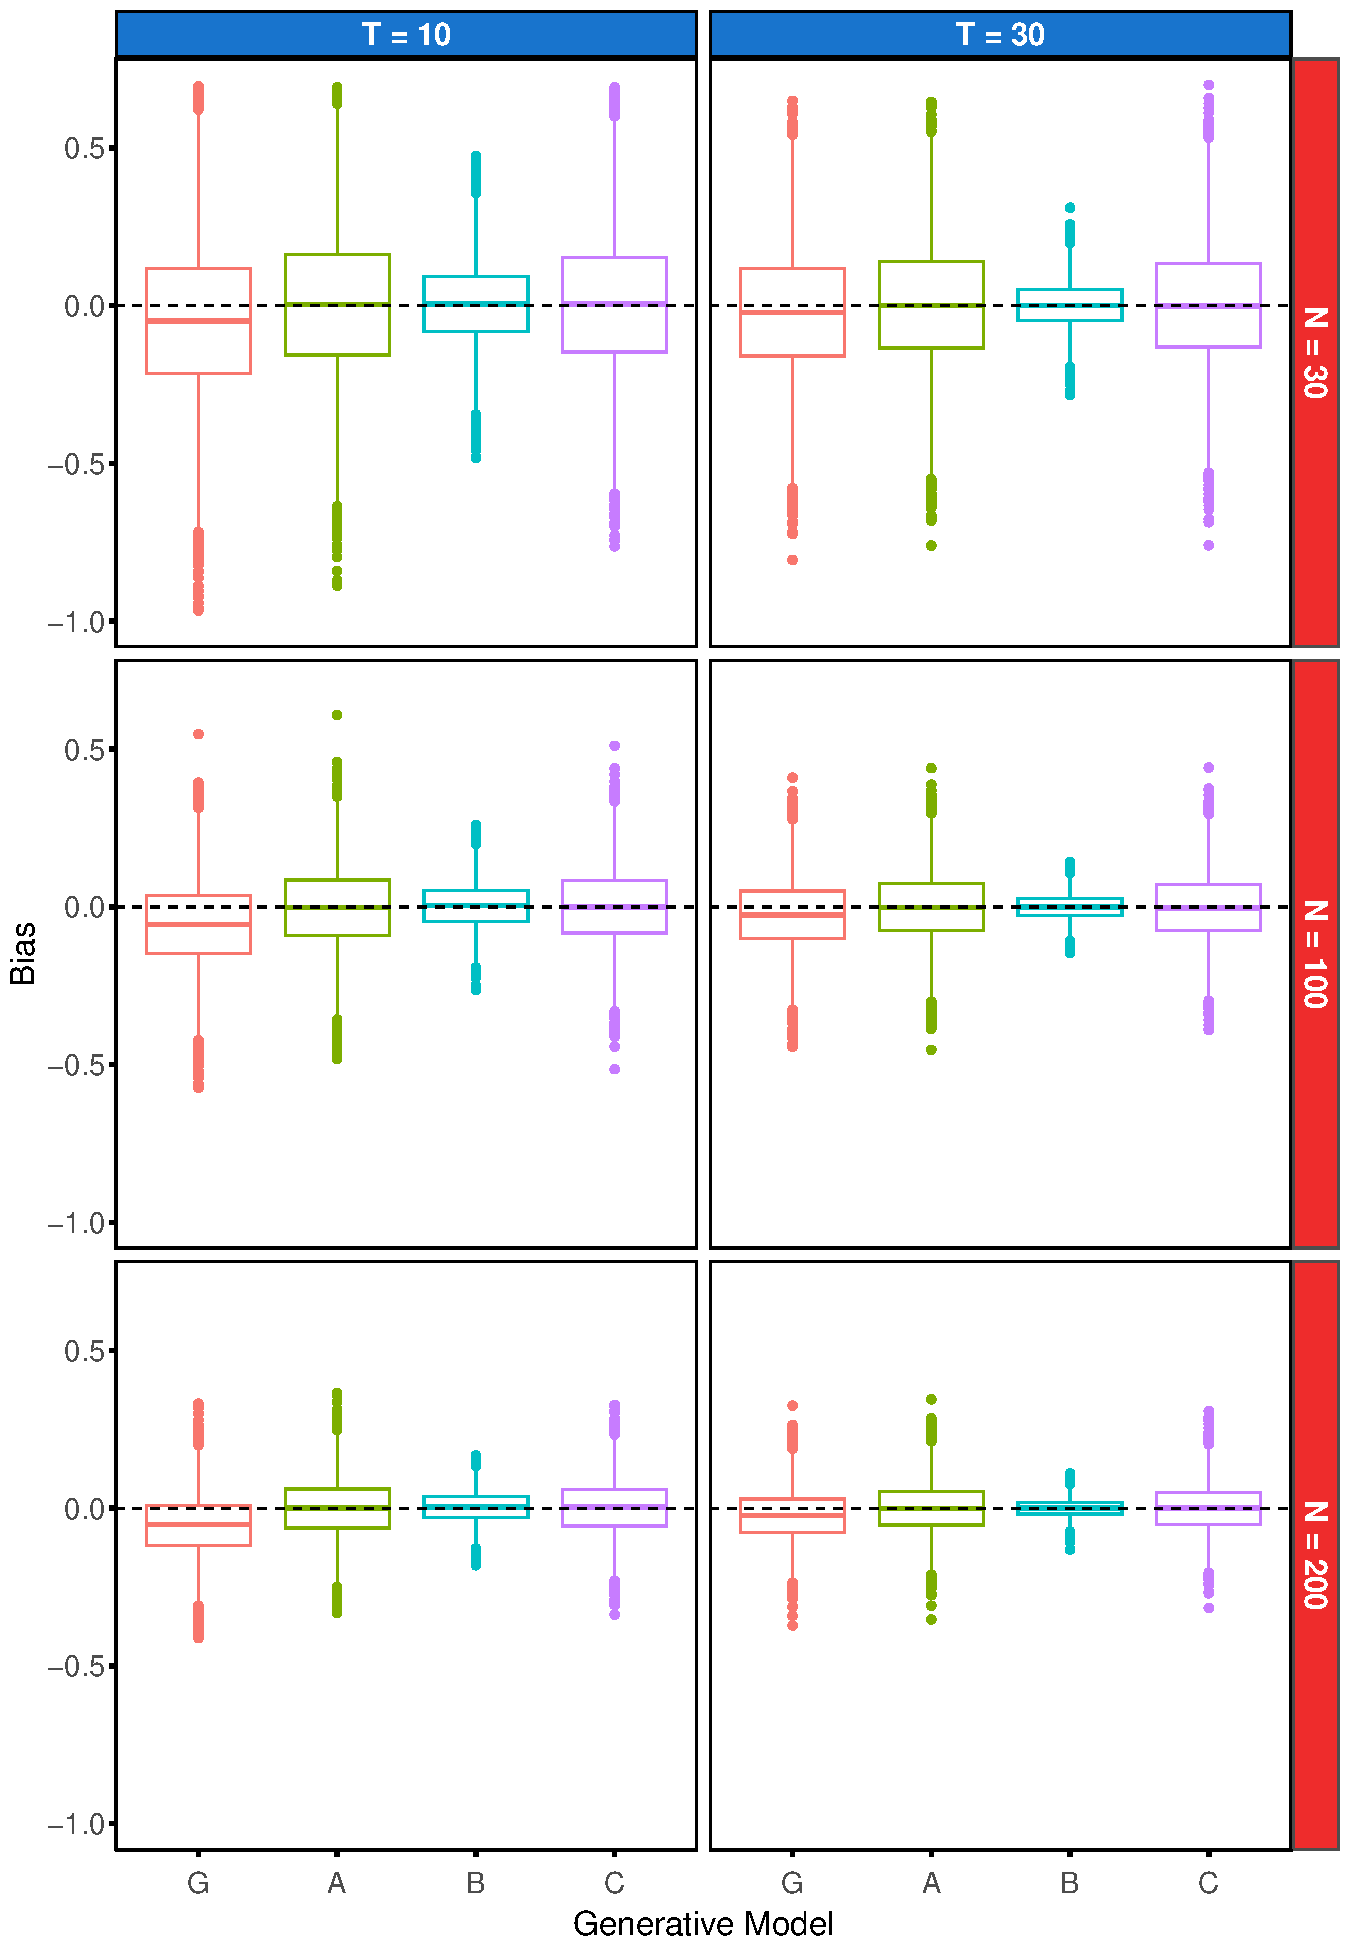
\includegraphics{research-report_files/figure-pdf/fig-simulation-results-1.pdf}

}

\end{minipage}%
%
\begin{minipage}{0.50\linewidth}

\subcaption{\label{fig-simulation-results-2}T=10, N=100}

\centering{

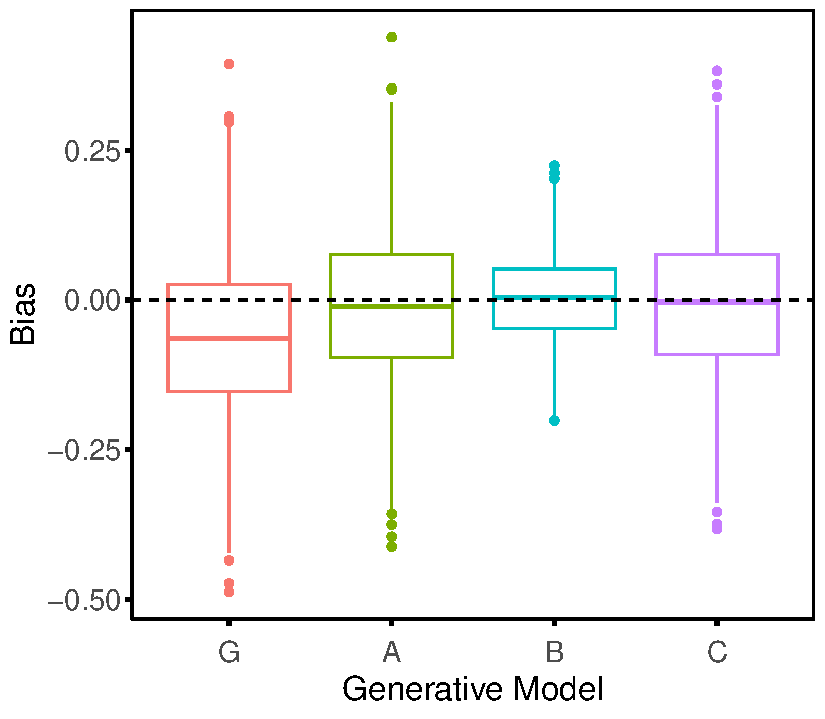
\includegraphics{research-report_files/figure-pdf/fig-simulation-results-2.pdf}

}

\end{minipage}%
\newline
\begin{minipage}{0.50\linewidth}

\subcaption{\label{fig-simulation-results-3}T=10, N=200}

\centering{

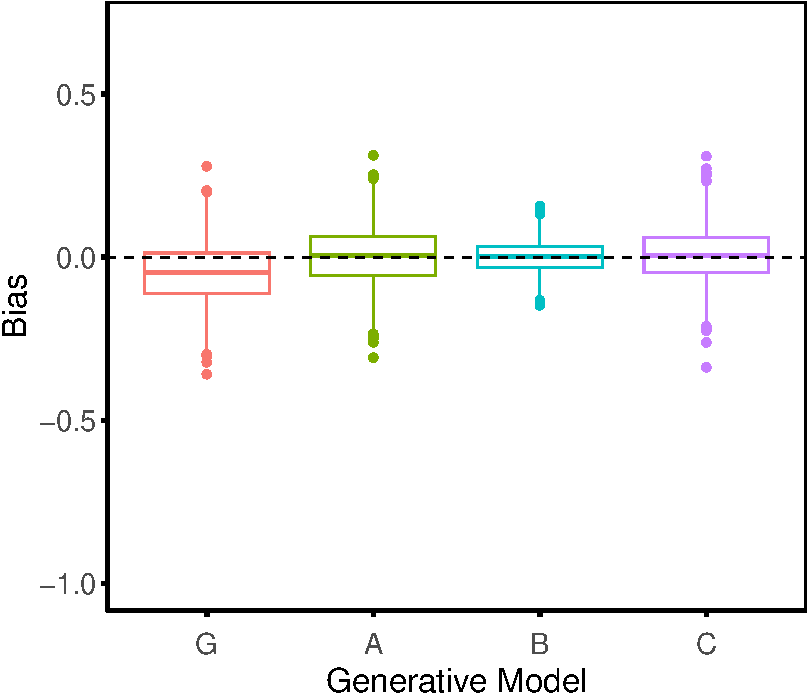
\includegraphics{research-report_files/figure-pdf/fig-simulation-results-3.pdf}

}

\end{minipage}%
%
\begin{minipage}{0.50\linewidth}

\subcaption{\label{fig-simulation-results-4}T=30, N=30}

\centering{

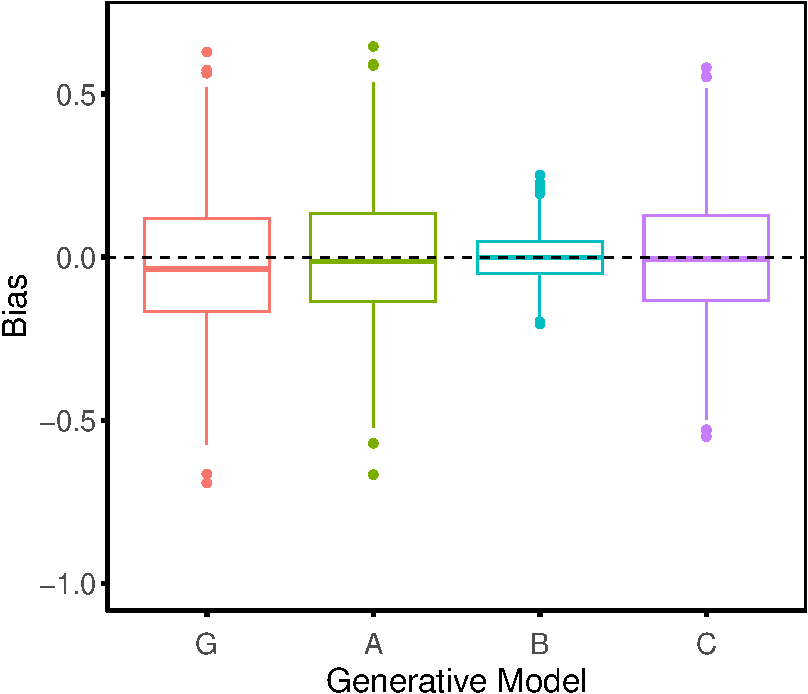
\includegraphics{research-report_files/figure-pdf/fig-simulation-results-4.pdf}

}

\end{minipage}%
\newline
\begin{minipage}{0.50\linewidth}

\subcaption{\label{fig-simulation-results-5}T=30, N=100}

\centering{

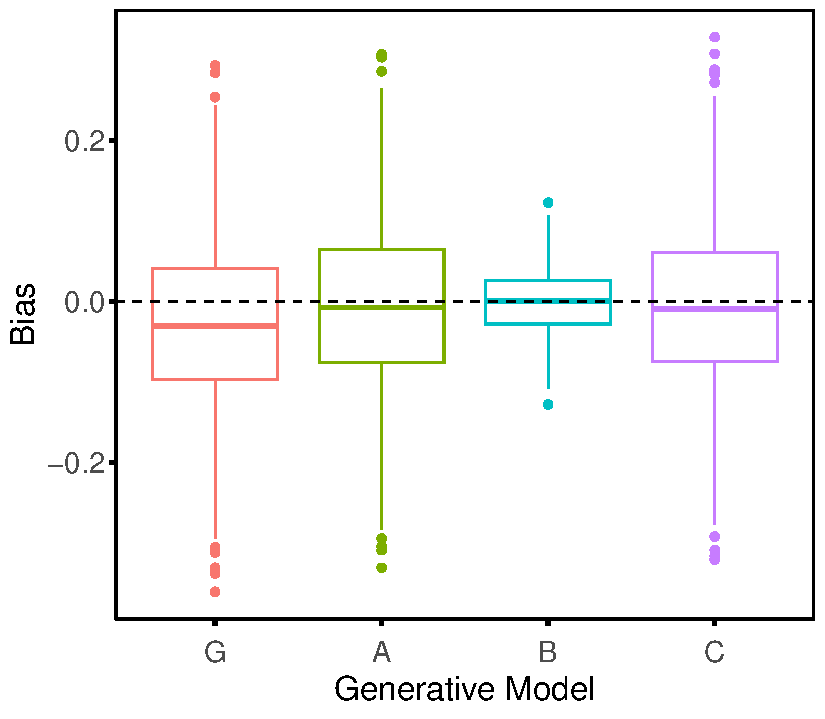
\includegraphics{research-report_files/figure-pdf/fig-simulation-results-5.pdf}

}

\end{minipage}%
%
\begin{minipage}{0.50\linewidth}

\subcaption{\label{fig-simulation-results-6}T=30, N=200}

\centering{

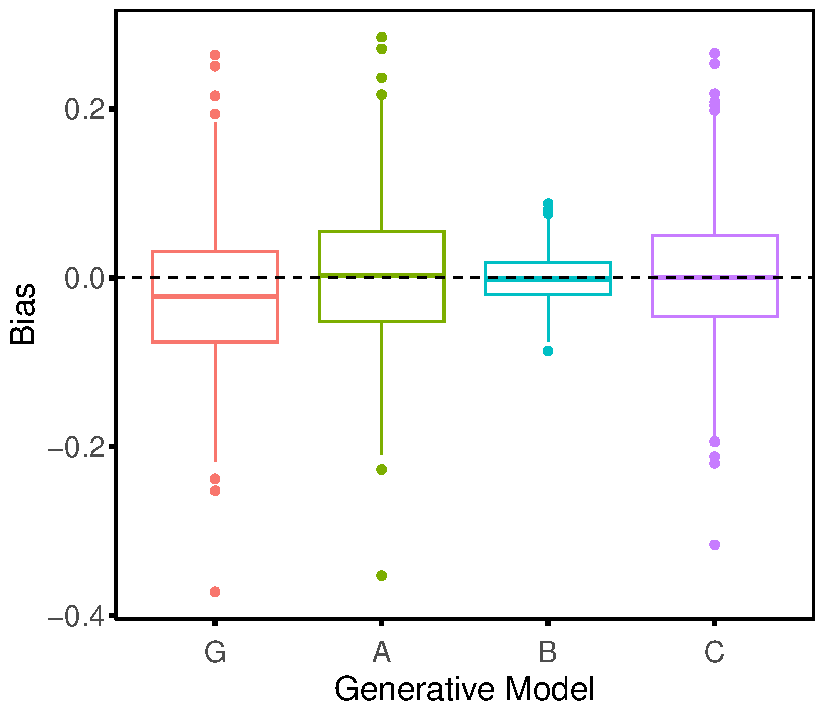
\includegraphics{research-report_files/figure-pdf/fig-simulation-results-6.pdf}

}

\end{minipage}%

\end{figure}%

In this reproduction of Qian et al. (\citeproc{ref-qian2020}{2020}), the
overall pattern was consistent with the original study (see
Figure~\ref{fig-simulation-results}): we observed substantial absolute
bias ranging from \(0.02\) to \(0.06\) for the most general generative
model (GM G), and much smaller bias of \(\leq 0.015\) for GM A. These
results align with expectations based on the conditional independence
assumption, which predicts that the treatment effect would be unbiased
for GM A and biased for GM G. However, the findings contradict the
backdoor criterion, which predicts no bias for any of the generative
models (GMs). Notably, we found greater treatment effect bias for GM A
than reported by Qian et al. (\citeproc{ref-qian2020}{2020}), with a
maximum bias of \(-0.012\) in the scenario with \(T = 10\) and
\(N = 100\) (see Table~\ref{tbl-simulation-results}), compared to
\(-0.003\) found by Qian et al. (\citeproc{ref-qian2020}{2020}) for the
same scenario. For GM G, the bias was most pronounced in this scenario
as well, reaching \(-0.064\). Furthermore, the size of the bias
decreased as the number of time points increased.

For the two additional special cases of GM G, namely GM B and GM C, we
observed even smaller absolute bias than for GM A: \(\leq 0.010\) for GM
C and \(\leq 0.005\) for GM B (see Table~\ref{tbl-simulation-results}).
These findings align with the backdoor criterion's prediction of no bias
but contradict the expectations based on the conditional independence
assumption, which suggests the presence of bias. Additionally, GM B
exhibited the smallest absolute bias overall and showed much smaller
variability across simulation replications compared to all other GMs. In
contrast, the remaining models exhibited comparable levels of
variability (see Figure~\ref{fig-simulation-results} and
Table~\ref{tbl-simulation-results}).

In summary, these findings suggest that once we modify the most general
model G by removing either the dependency of the random intercept on the
covariate (GM A), the random slope \(b_{i2}\) (GM B), or the interaction
term \(\beta_1\) (GM C), the bias either disappears or becomes
negligible. However, neither the backdoor criterion nor the conditional
independence assumption provided consistent predictions of treatment
effect bias across all models.

\section{Discussion}\label{discussion}

This report employed both graphical methods and data simulations to
understand and explain the issue of endogenous covariates.

While Qian et al. (\citeproc{ref-qian2020}{2020}) show that GM3 is the
only model with bias in the treatment effect, the backdoor criterion
failed to identify this bias, as there is no backdoor path in the
treatment effect. This may be explained by the fact that the classic DAG
does not impose restrictions based on (a) the random slopes and (b)
interaction effects.

The research question pertained to the extent of treatment effect bias
of generative models GM B and C that are special cases of GM G. First,
we reproduced the findings by Qian et al.
(\citeproc{ref-qian2020}{2020}) who found consistent estimators for GM1
and and inconsistent ones for GM3. Using additional generative models,
we found that bias became indiscernable when removing from GM3 either
the dependency between the random intercept and covariate (GM1), the
random slope for treatment (GM3A) or the interaction effect (GM3B). This
finding is in sharp contrast to the suggestion of the conditional
independence assumption that the treatment effect would be biased for
GM3, 3A and 3B.

The current research report leaves several avenues unexplored. First, it
is unclear whether the simulation findings pertaining the generative
models in Qian et al. (\citeproc{ref-qian2020}{2020}) and here
generalize to other generative models. For instance, we found here that
removal of a random slope or interaction from GM3 got rid of most if not
all of the treatment effect bias. Thus, it is important to establish how
this generalizes, so that practical recommendations can be formulated.
This is particularly important, since while violations of model
assumptions are never desired, the robustness against and the practical
implications of a violation is what matters. Second, it is unclear how
exactly the divide between the literatures pertaining to the focus of
the MLM on different centering methods and within- and between-person
interpretations and the focus of the GEE on marginal and conditional
interpretations may be bridged. Consequently, future research could
assess the implications of centering methods in MLMs on the extent to
which the marginal interpretation of MLM breaks down. Third, we found
that the classical DAG may not be sufficient to identify bias in the
treatment effect for GM3, especially due to its lack of specification of
interaction effects. Concerns regarding the use of Pearl's backdoor
criterion in situations with interaction effects have been voiced by
several people (see Weinberg (\citeproc{ref-weinberg2007}{2007}); Attia
et al. (\citeproc{ref-attia2022}{2022})). Future research could explore
to what extent proposed extensions of the DAG may be useful in
identifying bias in the treatment effect for GM3. Finally, it may be
interesting to investigate the implications of endogenous covariates in
MLMs for other types of longitudinal data analysis methods, such as
dynamic structural equation modelling (DSEM; a widely used framework in
the social sciences based on MLM).

Third, since the issue extends to all longitudinal data analysis methods
according to Diggle (\citeproc{ref-diggle2002}{2002}), in future
research it may be interesting to investigate the implications of
endogenous covariates in MLMs for other types of longitudinal data
analysis methods, such as dynamic structural equation modelling (DSEM; a
widely used framework in the social sciences based on MLM).

\textbf{to recognize and understand precisely when and why endogenous
covariates may trouble an empirical investigation.}

\newpage

\section{References}\label{references}

\phantomsection\label{refs}
\begin{CSLReferences}{1}{0}
\bibitem[\citeproctext]{ref-attia2022}
Attia, J., Holliday, E., \& Oldmeadow, C. (2022). A proposal for
capturing interaction and effect modification using DAGs.
\emph{International Journal of Epidemiology}, \emph{51}(4), 1047--1053.
\url{https://doi.org/10.1093/ije/dyac126}

\bibitem[\citeproctext]{ref-bates2015}
Bates, D., Mächler, M., Bolker, B., \& Walker, S. (2015). Fitting linear
mixed-effects models using {lme4}. \emph{Journal of Statistical
Software}, \emph{67}(1), 148.
\url{https://doi.org/10.18637/jss.v067.i01}

\bibitem[\citeproctext]{ref-bauer2011}
Bauer, D. J., \& Sterba, S. K. (2011). Fitting multilevel models with
ordinal outcomes: Performance of alternative specifications and methods
of estimation. \emph{Psychological Methods}, \emph{16}(4), 373--390.
\url{https://doi.org/10.1037/a0025813}

\bibitem[\citeproctext]{ref-daniel2013}
Daniel, R. m., Cousens, S. n., De Stavola, B. l., Kenward, M. G., \&
Sterne, J. a. C. (2013). Methods for dealing with time-dependent
confounding. \emph{Statistics in Medicine}, \emph{32}(9), 1584--1618.
\url{https://doi.org/10.1002/sim.5686}

\bibitem[\citeproctext]{ref-diggle2002}
Diggle, P. (2002). \emph{Analysis of Longitudinal Data}. OUP Oxford.

\bibitem[\citeproctext]{ref-duncan1966}
Duncan, O. D. (1966). Path analysis: Sociological examples.
\emph{American Journal of Sociology}, \emph{72}(1), 1--16.
\url{https://doi.org/10.1086/224256}

\bibitem[\citeproctext]{ref-elwert2014}
Elwert, F., \& Winship, C. (2014). Endogenous selection bias: The
problem of conditioning on a collider variable. \emph{Annual Review of
Sociology}, \emph{40}, 31--53.
\url{https://doi.org/10.1146/annurev-soc-071913-043455}

\bibitem[\citeproctext]{ref-hamaker2020}
Hamaker, E. L., \& Muthén, B. (2020). The fixed versus random effects
debate and how it relates to centering in multilevel modeling.
\emph{Psychological Methods}, \emph{25}(3), 365--379.
\url{https://doi.org/10.1037/met0000239}

\bibitem[\citeproctext]{ref-Holland1986}
Holland, P. W. (1986). Statistics and causal inference. \emph{Journal of
the American Statistical Association}, \emph{81}(396), 945--960.
\url{https://doi.org/10.2307/2289064}

\bibitem[\citeproctext]{ref-Kim2021a}
Kim, Y., \& Steiner, P. M. (2021). Causal graphical views of fixed
effects and random effects models. \emph{British Journal of Mathematical
and Statistical Psychology}, \emph{74}(2), 165--183.
\url{https://doi.org/10.1111/bmsp.12217}

\bibitem[\citeproctext]{ref-nahum-shani2021}
Nahum-Shani, I., Potter, L. N., Lam, C. Y., Yap, J., Moreno, A.,
Stoffel, R., Wu, Z., Wan, N., Dempsey, W., Kumar, S., \& al., et.
(2021). The mobile assistance for regulating smoking (MARS)
micro-randomized trial design protocol. \emph{Contemporary Clinical
Trials}, \emph{110}, 106513.
\url{https://doi.org/10.1016/j.cct.2021.106513}

\bibitem[\citeproctext]{ref-pearl1988}
Pearl, J. (1988). \emph{Probabilistic Reasoning in Intelligent Systems:
Networks of Plausible Inference}. Morgan Kaufmann.

\bibitem[\citeproctext]{ref-pearl1995}
Pearl, J. (1995). Causal diagrams for empirical research.
\emph{Biometrika}, \emph{82}(4), 669--688.
\url{https://doi.org/10.1093/biomet/82.4.669}

\bibitem[\citeproctext]{ref-pearl2009}
Pearl, J. (2009). \emph{Causality: Models, reasoning, and inference}
(2nd ed.). Cambridge University Press.

\bibitem[\citeproctext]{ref-qian2020}
Qian, T., Klasnja, P., \& Murphy, S. A. (2020). Linear mixed models with
endogenous covariates: Modeling sequential treatment effects with
application to a mobile health study. \emph{Statistical Science : A
Review Journal of the Institute of Mathematical Statistics},
\emph{35}(3), 375--390. \url{https://doi.org/10.1214/19-sts720}

\bibitem[\citeproctext]{ref-raudenbush2002}
Raudenbush, S. W., \& Bryk, A. S. (2002). \emph{Hierarchical Linear
Models: Applications and Data Analysis Methods} (2nd ed.). SAGE.

\bibitem[\citeproctext]{ref-Schoot2017}
Schoot, J. H. M. M. R. van de. (2017). \emph{Multilevel analysis:
Techniques and applications, third edition} (3rd ed.). Routledge.
\url{https://doi.org/10.4324/9781315650982}

\bibitem[\citeproctext]{ref-rcoreteam2024}
Team, R. C. (2024). \emph{R: A language and environment for statistical
computing}. R Foundation for Statistical Computing.
\url{https://www.R-project.org/}

\bibitem[\citeproctext]{ref-walton2018}
Walton, A., Nahum-Shani, I., Crosby, L., Klasnja, P., \& Murphy, S.
(2018). Optimizing digital integrated care via micro-randomized trials.
\emph{Clinical Pharmacology \& Therapeutics}, \emph{104}(1), 53--58.
\url{https://doi.org/10.1002/cpt.1079}

\bibitem[\citeproctext]{ref-weinberg2007}
Weinberg, C. R. (2007). Commentary: Can DAGs clarify effect
modification? \emph{Epidemiology}, \emph{18}(5), 569--572.
\url{https://www.jstor.org/stable/20486428}

\bibitem[\citeproctext]{ref-Wodtke2020}
Wodtke, G. T. (2020). Regression-based adjustment for time-varying
confounders. \emph{Sociological Methods \& Research}, \emph{49}(4),
906--946. \url{https://doi.org/10.1177/0049124118769087}

\bibitem[\citeproctext]{ref-wright1934a}
Wright, S. (1934). The method of path coefficients. \emph{The Annals of
Mathematical Statistics}, \emph{5}(3), 161--215.
\url{https://doi.org/10.1214/aoms/1177732676}

\end{CSLReferences}




\end{document}
